\documentclass[a4paper, 12pt]{report}

\usepackage{amsmath}
\usepackage{esint}
\usepackage{comment}
\usepackage{amssymb}
\usepackage{commath}
\usepackage{geometry}
\usepackage{graphicx}
\usepackage{hyperref}
\usepackage{listings}
\usepackage{xcolor}
\usepackage{array}
\usepackage{longtable}

\definecolor{codegreen}{rgb}{0,0.6,0}
\definecolor{codegray}{rgb}{0.5,0.5,0.5}
\definecolor{codepurple}{rgb}{0.58,0,0.82}
\definecolor{backcolour}{rgb}{0.95,0.95,0.92}

\def\t{\theta}
\def\a{\alpha}
\def\be{\beta}
\def\w{\omega}
\def\la{\lambda}
\def\g{\gamma}
\def\f{\frac}
\def\l{\left}
\def\r{\right}
\def\dst{\displaystyle}
\def\b{\bar}
\def\h{\hat}
\def\ph{\phi}
\def\d{\cdot}
\def\n{\nabla}
\def\p{\partial}
\def\lap{\mathcal{L}}
\def\sizem{0.93}
\def\size{0.75}
\def\tabsize{4.4cm}
\def\stabsize{0.97cm}
\def\mtabsize{0.73cm}
\def\ltabsize{5.5cm}

%\let\stdsection\section
%\renewcommand\section{\newpage\stdsection}
\geometry{portrait, margin= 0.7in}

\begin{document}

\title{Automated Convergence Testing}
\author{Hans C. Suganda}
\date{$25^{th}$ November 2021}
\maketitle
\newpage

\lstset{
	columns=fullflexible,
	frame=single,
	breaklines=true,
	backgroundcolor=\color{backcolour},   
	commentstyle=\color{codegreen},
	keywordstyle=\color{magenta},
	numberstyle=\tiny\color{codegray},
	stringstyle=\color{codepurple},
	basicstyle=\ttfamily\footnotesize,
	keepspaces=true,                 
	numbersep=5pt,                  
	showspaces=false,               
	showtabs=false,                  
	tabsize=2
}

\tableofcontents
\newpage

\begin{center}
\begin{comment}
Tasks to do:

Find out how to change the overrelaxation parameter (Priority)
    Make a simple NN model,
    Make some easy test cases,
    See if overrelaxaition parameter is succesful

Run the automated Script again with the following specifications:
Width: 100 -> 200, step size 20
Depth: 1 -> 8, step size 1
    Fix The l^2 Error, find the mean of the current one
        Fetch the expression for RMSE,
        Fix Algorithm
        Run for Test Case and Verify Fix is succesful
    Run the conditions
        Might Either Run Locally or use One of the Clusters to run it


Find a way to test the epoch to convergence by examining history
    For a relatively medium sized model, say width 80 and depth 3, plot history.dat
    Determine what "Convergence constitutes"


Read the paper given

Meet at December 2^nd

\end{comment}
%Seperator
%Seperator
%Seperator
\section{Modifying Learning Rate}
\begin{comment}
\end{comment}
%Seperator
%Seperator
\subsection{Simple Learning Case}
The python script below \url{Simple_NN.py} shows how the learning rate can be changed dynamically (at runtime). \url{Simple_NN.py} generates a neural network with $3$ input nodes, $3$ output nodes and $2$ hidden lyaers of $4$ nodes with sigmoid activation functions. The input data and output data does not matter, neither does the performance of the neural network. What is being demonstrated is how dynamic learning rate can be implemented,
\begin{lstlisting}[language=python]
import numpy as np
import tensorflow as tf
from tensorflow import keras
from tensorflow.keras import layers
import matplotlib.pyplot as plt

#Training Numbers
trainum = 1000

#Training Inputs
traininputs = np.array([
    [1.0,0.0,0.0],
    [0.0,1.0,0.0],
    [0.0,0.0,1.0]
])

#Training Outputs
trainoutputs = np.array([
    [0.0,1.0,0.0],
    [1.0,0.0,0.0],
    [0.0,0.0,1.0]
])

#Defining Inputs of Neural Network
inputs = tf.keras.Input(shape=(3))

#Some Arbitrary Neural Network Architecture
layer1 = tf.keras.layers.Dense(4, activation='sigmoid')(inputs)
layer2 = tf.keras.layers.Dense(4, activation='sigmoid')(layer1)

#Defining Outputs of Neural Network
outputs = tf.keras.layers.Dense(3)(layer2)

#Defining Model used
model = tf.keras.Model(inputs = inputs, outputs = outputs)

#Determine the Learning Rate
lr_schedule = keras.optimizers.schedules.ExponentialDecay(
    initial_learning_rate=1e-2,
    decay_steps=10000,
    decay_rate=0.2)

#Show the Decaying Learning Rate
def get_lr_metric(optimizer):
    def lr(y_true, y_pred):
        return optimizer._decayed_lr(tf.float32)
    return lr

#Instantiate an optimizer
opt = tf.keras.optimizers.Adam(learning_rate = lr_schedule)
lr_metric = get_lr_metric(opt)

#Compile Model
model.compile(
    optimizer = opt,
    metrics=['accuracy', lr_metric],
    loss='mean_squared_error')

#Train Model
model.fit(
    x=traininputs, 
    y=trainoutputs, 
    batch_size=None,
    epochs = trainum
)

#Testing the model
print(model(traininputs))

#Customary End
print('Leaves Blow in the Wind...')
\end{lstlisting}
$$$$
The process is described below:
\begin{itemize}
\item Instantiate a learning rate scheduler (\url{lr_schedule})
\item Define a function that calls a method in optimizer class for learning rate (\url{get_lr_metric})
\item Instantiate optimizer (\url{opt})
\item Declare a variable (\url{lr_metric}) which is the said function (\url{get_lr_metric}) acting on the instantiated optimizer (\url{opt})
\item Compile model while passing an additional metric (\url{lr_metric})
\end{itemize}
$$$$
The resulting output of the neural network being trained by \url{Simple_NN.py} showing the learning rate changing dynamically (at runtime),
\begin{lstlisting}
Epoch 157/1000
1/1 [==============================] - 0s 14ms/step - loss: 0.0349 - accuracy: 1.0000 - lr: 0.0098
Epoch 158/1000
1/1 [==============================] - 0s 7ms/step - loss: 0.0336 - accuracy: 1.0000 - lr: 0.0097
Epoch 159/1000
1/1 [==============================] - 0s 16ms/step - loss: 0.0322 - accuracy: 1.0000 - lr: 0.0097
\end{lstlisting}
$$$$
%Seperator
%Seperator
\subsection{Implementation to Helmholtz Script}
The learning rate and the function is declared at the \url{NN Parameters} section,
\begin{lstlisting}[language=python]
#Loop to build Architecture
for x in range(0, depth):
    layers.append(width)  
    activations.append('tanh')

#Appending Last Element
layers.append(1) 
activations.append('linear')

#Determine the Learning Rate
lr_schedule = keras.optimizers.schedules.ExponentialDecay(
    initial_learning_rate=1e-2,
    decay_steps=10000,
    decay_rate=0.2)

#Show the Decaying Learning Rate
def get_lr_metric(optimizer):
    def lr(y_true, y_pred):
        return optimizer._decayed_lr(tf.float32) # I use ._decayed_lr method instead of .lr
    return lr
\end{lstlisting}
$$$$
The \url{build_model} function is altered slightly to implement the changes described in the previous subsection,
\begin{lstlisting}[language=python]
    # compile model
    # Instantiate an optimizer
    opt = tf.keras.optimizers.Adam(learning_rate = lr_schedule)
    lr_metric = get_lr_metric(opt)
    my_model.compile(optimizer= opt,
                     loss=loss_func_list, loss_weights = loss_weight_list,
                     metrics=['accuracy', lr_metric])
    return my_model
\end{lstlisting}
$$$$
However, this results in an error early in \url{main}. This error could be "fixed" by commenting out the following lines,
\begin{lstlisting}[language=python]
    #default_lr = get_learning_rate(the_DNN)
    #print("Default learning rate: %f" % default_lr)
    #if LR_factor > 1.0 or LR_factor < 1.0:
    #    LR = LR_factor * default_lr
    #    set_learning_rate(the_DNN, LR)
    #else:
    #    LR = default_lr
\end{lstlisting}
$$$$
The resulting output showing the learning rate changing dynamically for the Helmholtz script,
\begin{lstlisting}
Epoch 285/50000
1/1 [==============================] - 0s 10ms/step - loss: 825.3599 - accuracy: 0.0000e+00 - lr: 0.0096
Epoch 286/50000
1/1 [==============================] - 0s 6ms/step - loss: 825.3511 - accuracy: 0.0000e+00 - lr: 0.0096
Epoch 287/50000
1/1 [==============================] - 0s 6ms/step - loss: 825.3417 - accuracy: 0.0000e+00 - lr: 0.0095
Epoch 288/50000
1/1 [==============================] - 0s 5ms/step - loss: 825.3316 - accuracy: 0.0000e+00 - lr: 0.0095
\end{lstlisting}
%Seperator
%Seperator
%Seperator
\section{Convergence Criteria}
\begin{comment}
\end{comment}
Convergence is important in considering whether the errors of the model could be attributed mostly to the architecture of the neural network or the lack of sufficient training. To make meaningful comparisons, it is important to decide what constitutes "convergence" of the model used. Since convergence is a loosely defined term and can be defined in multiple ways, below describes one criteria implemented in this study.
%Seperator
%Seperator
\subsection{Theoretical Criteria}
Suppose $x$ is some variable that varies with numbers of computer iterations $n$, wherein $n$ is some integer. Let the finite difference of $x$ between a particular index $p$ and $p+\a$ be defined as,
$$\Delta x = x(p+\a) - x(p)$$
Typically, the loss function varies with training iterations as shown below,
\\~\\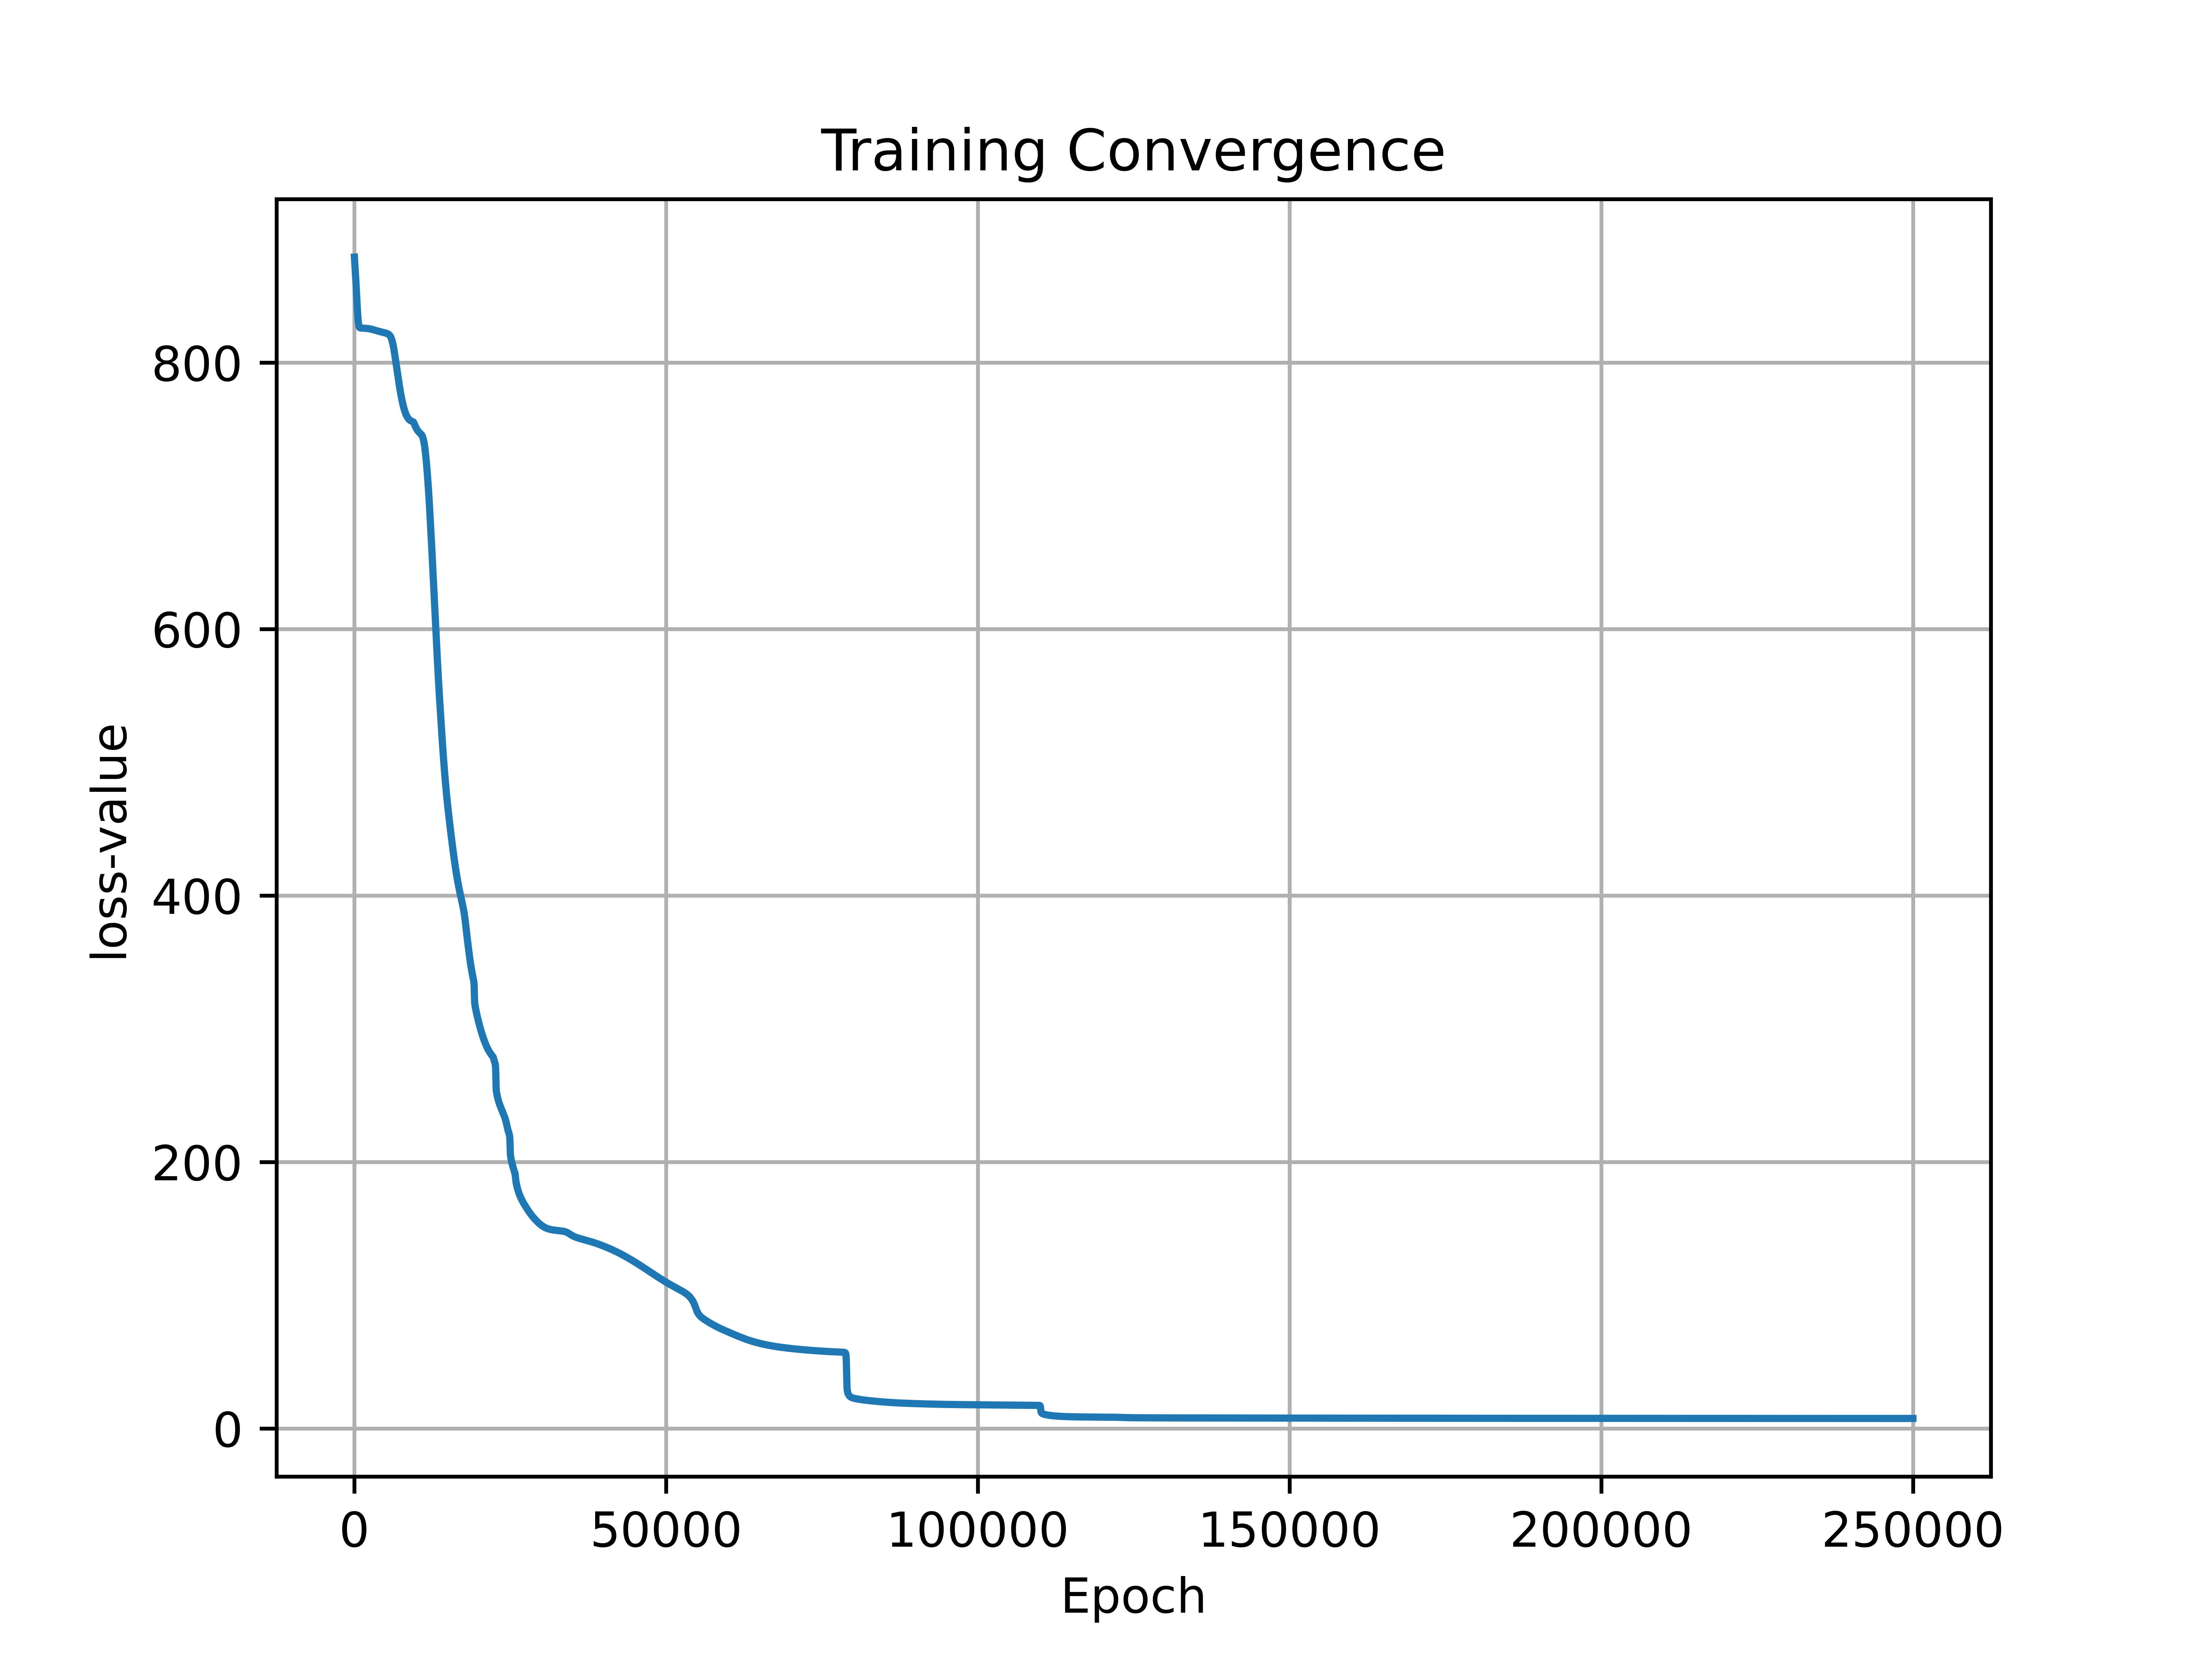
\includegraphics[scale=\sizem]{Train_Convergence.png}
\\~\\This is the training curve for a neural network with $2$ hidden layers with $20$ nodes each solving the Helmholtz equation. Notice the characteristic "L" of the curve. The loss function changes drastically and quickly for the first $50000$ iterations but change very slowly in the last $50000$ training iterations. If this can be considered as the typical behaviour of a converged neural network, then convergence can be decided on the rate of change of loss function near the end of the training iteration when compared to the start of the training iterations. Motivated by this, let convergence be defined as
$$|x(n) - x((k_1-1)n)| < |\epsilon[x(k_2 n) - x(1)]|$$
wherein $0<k_1,k_2,\epsilon<1$. If the loss function does not change too much near the end of the training iterations compared to the change of the loss function at the beginning of the training iterations, then the neural network is assumed to be "converged". $\epsilon$, $k_1$ and $k_2$ are all parameters that controls how "sharp" the "L" shape must be in order for the convergence critertion to hold true. 
%Seperator
%Seperator
\subsection{Programming Implementation}
The python script \url{convergence.py} reads a numpy array and determines convergence based on the criteria mentioned above,
\begin{lstlisting}[language=python]
#Author: Hans C. Suganda
import numpy as np

"""
ind represents the independent variable, which should be a numpy array. To test for convergence, the function below takes average gradient at the earlier stages of the given array. The function does the same but for later stages of the given array, then if the gradient at the later stages of the array is much less than the initial gradient, then the given array is assumed to have indicated "convergence" of the numerical scheme
"""

def run(ind):
    cutoff = 0.03 #Allowable percentage difference of the gradients
    percfront = 0.2 #percentage from the front for the index
    percback = 0.3 #percentage from the back for the index
    elsize = ind.size #Necessary for indexing
    
    #Initial Gradient
    gradinit = ind[int(elsize*percfront)] - ind[0]
    
    #Final Gradient
    gradfin = ind[elsize-1] - ind[int(elsize*(1.0-percback))]

    #Convergence Criterion
    result = False
    if(abs(gradfin)<(cutoff*abs(gradinit))):
        result = True
    
    return result
\end{lstlisting}

%Seperator
%Seperator
%Seperator
\section{Automated Testing Results}
\begin{comment}
\end{comment}
%Seperator
%Seperator
\subsection{Plotting Algorithm}
The python script below collects all the various history files and plots the loss function as a variation of training iterations in one file,
\begin{lstlisting}[language=python]
#Author: Hans C. Suganda
import numpy as np
import matplotlib.pyplot as plt
import glob

#Files to Open
filename_list = glob.glob('*_120_*.csv')

#Plotting
plt.figure()
for filename in filename_list:
    data = np.genfromtxt(filename, delimiter=',', comments=",loss,")
    plt.plot(data[:,0], data[:,1], label = filename)
plt.xlabel('Epochs')
plt.ylabel('loss-value')
plt.title('Training Convergence')
plt.legend()
plt.grid()

#Show Plot
plt.show()
\end{lstlisting}
%Seperator
%Seperator
\newpage
\subsection{Plots Across Constant Width}
%Seperator
\subsubsection{30 Nodes}
When the hidden layers each have $30$ nodes, an overview of the training curve is shown below,
\\~\\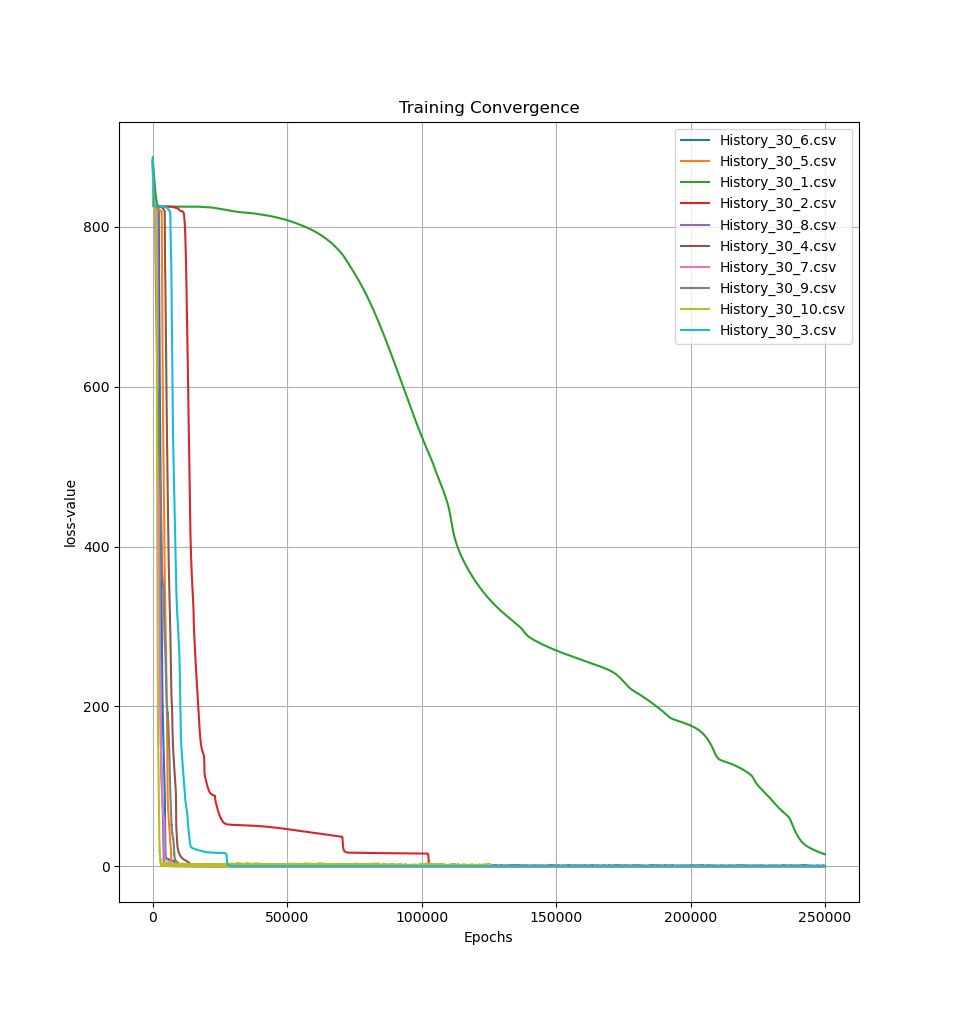
\includegraphics[scale=\size]{Width_30_Overview.png}
\newpage
At the beginning of the training iterations,
\\~\\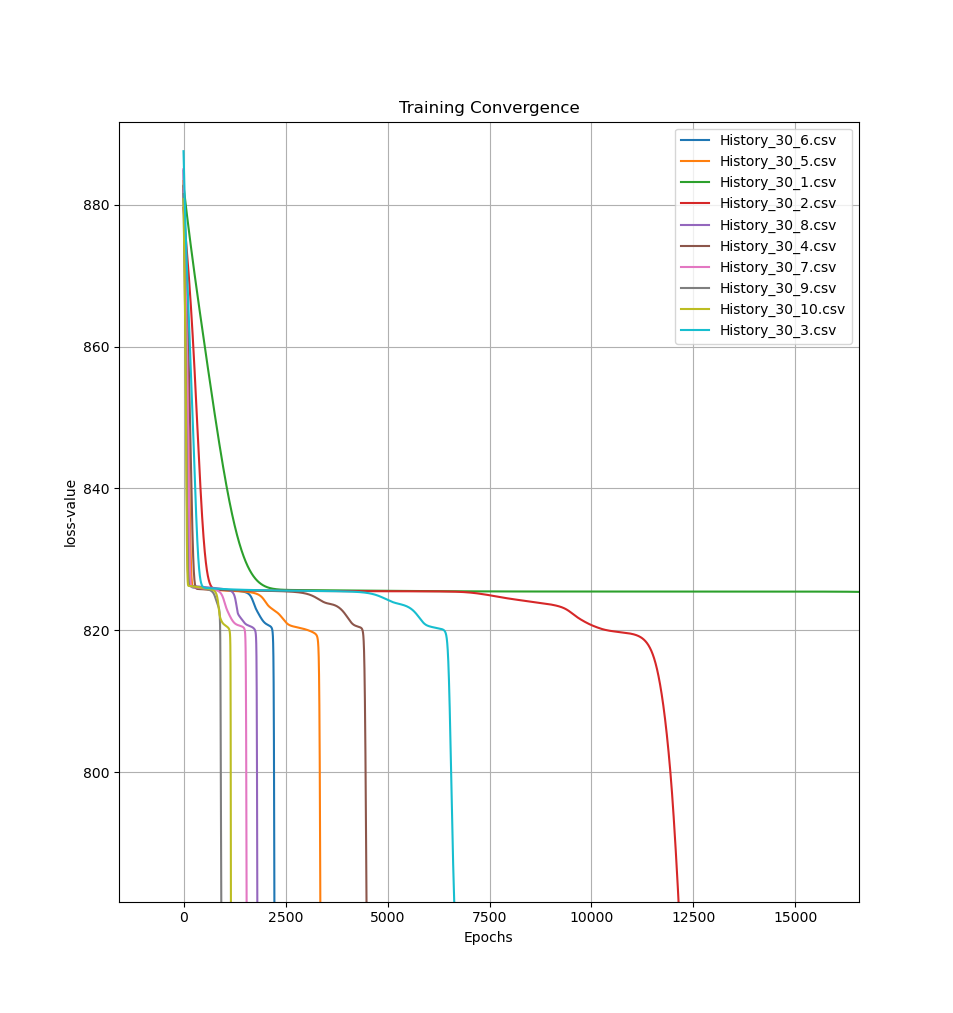
\includegraphics[scale=\size]{Width_30_Beginning.png}
\newpage
For the regions where many of the cases have converged,
\\~\\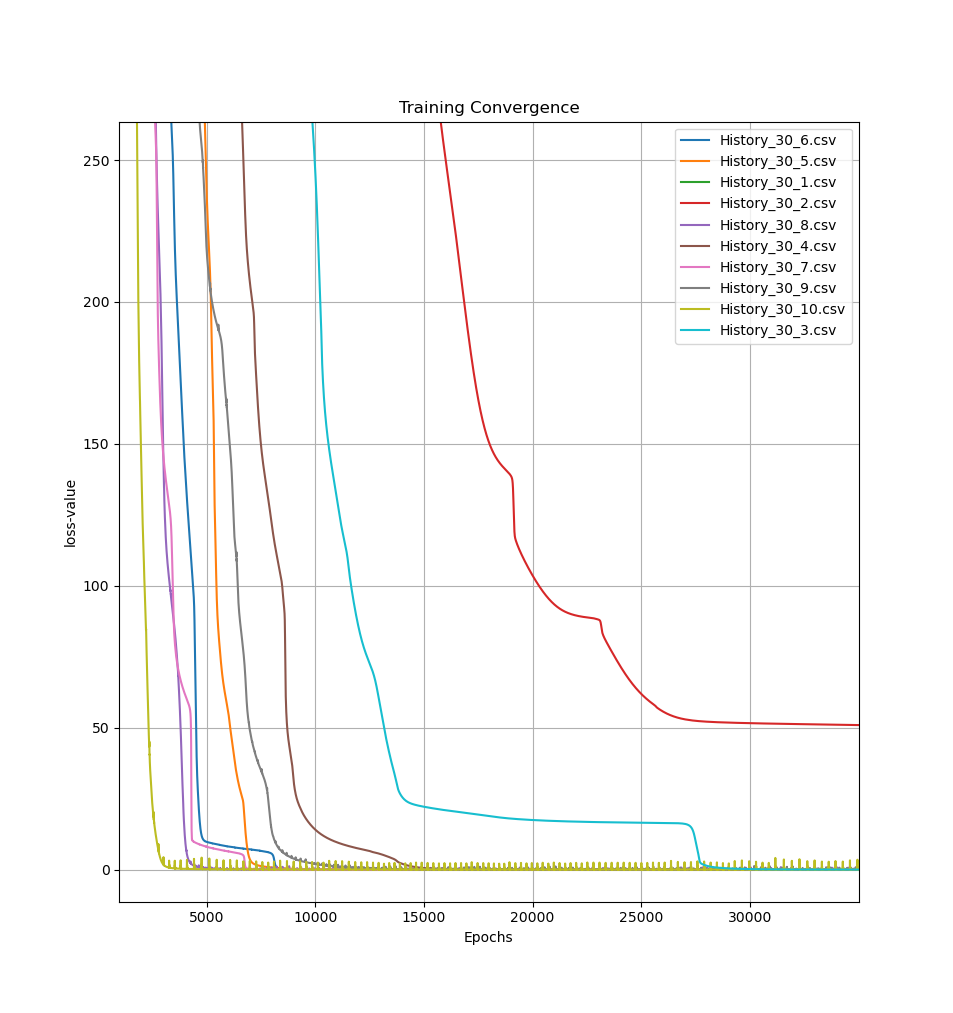
\includegraphics[scale=\size]{Width_30_Down.png}
%Seperator
\newpage
\subsubsection{100 Nodes}
When the hidden layers each have $100$ nodes, an overview of the training curve is shown below,
\\~\\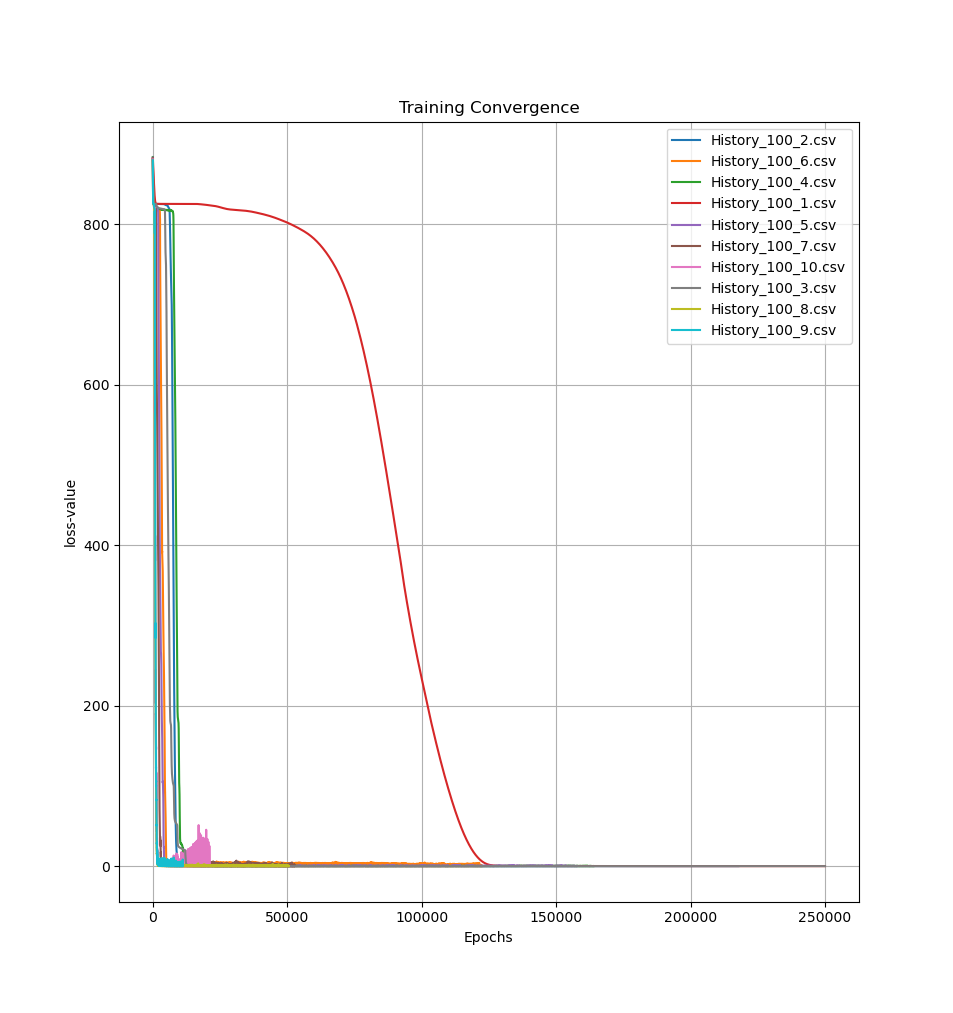
\includegraphics[scale=\size]{Width_100_Overview.png}
\newpage
At the beginning of the training iterations,
\\~\\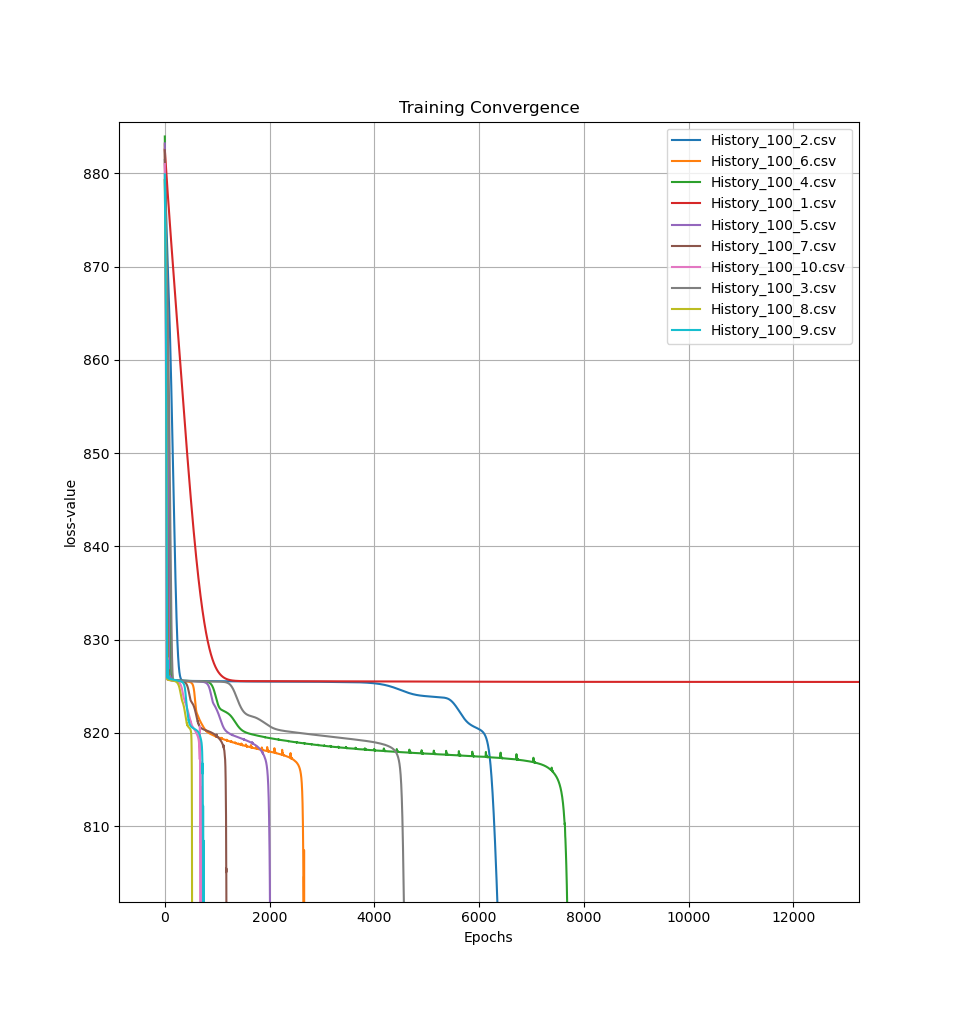
\includegraphics[scale=\size]{Width_100_Beginning.png}
\newpage
For the regions where many of the cases have converged,
\\~\\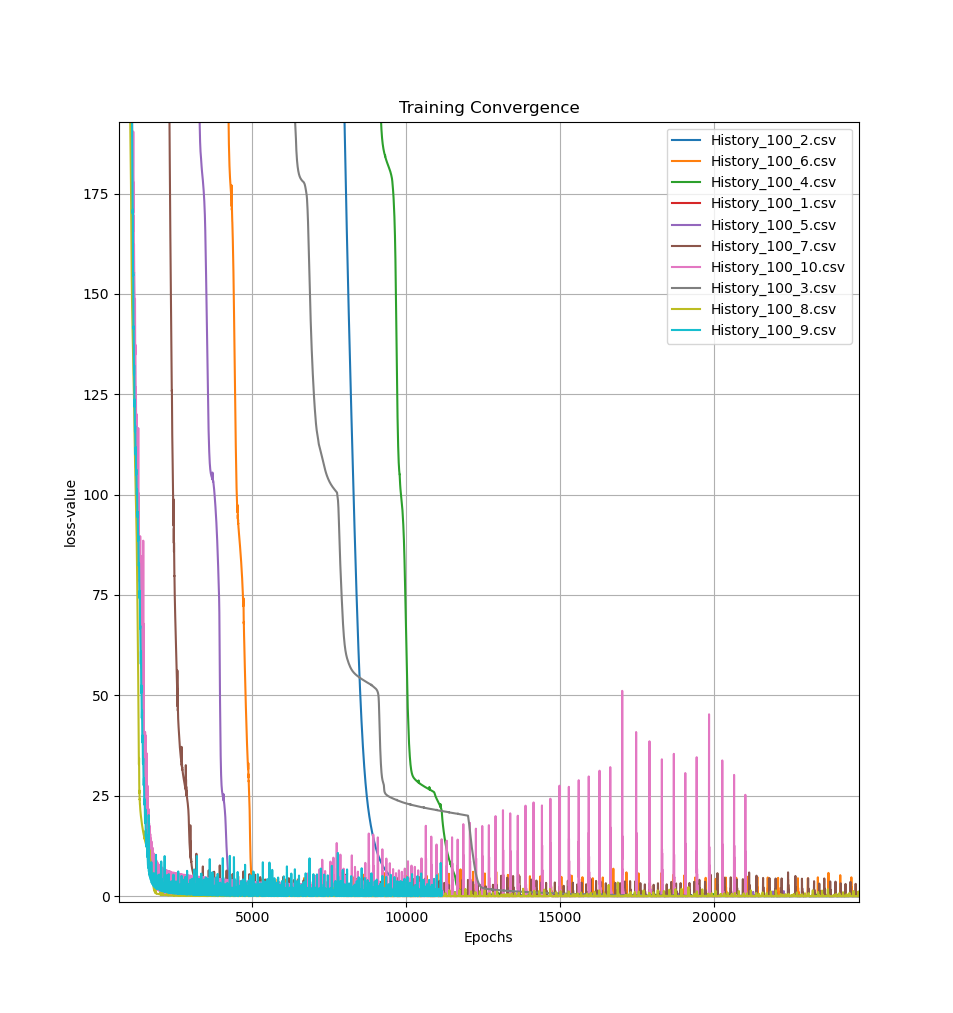
\includegraphics[scale=\size]{Width_100_Down.png}
%Seperator
\newpage
\subsubsection{180 Nodes}
When the hidden layers each have $180$ nodes, an overview of the training curve is shown below,
\\~\\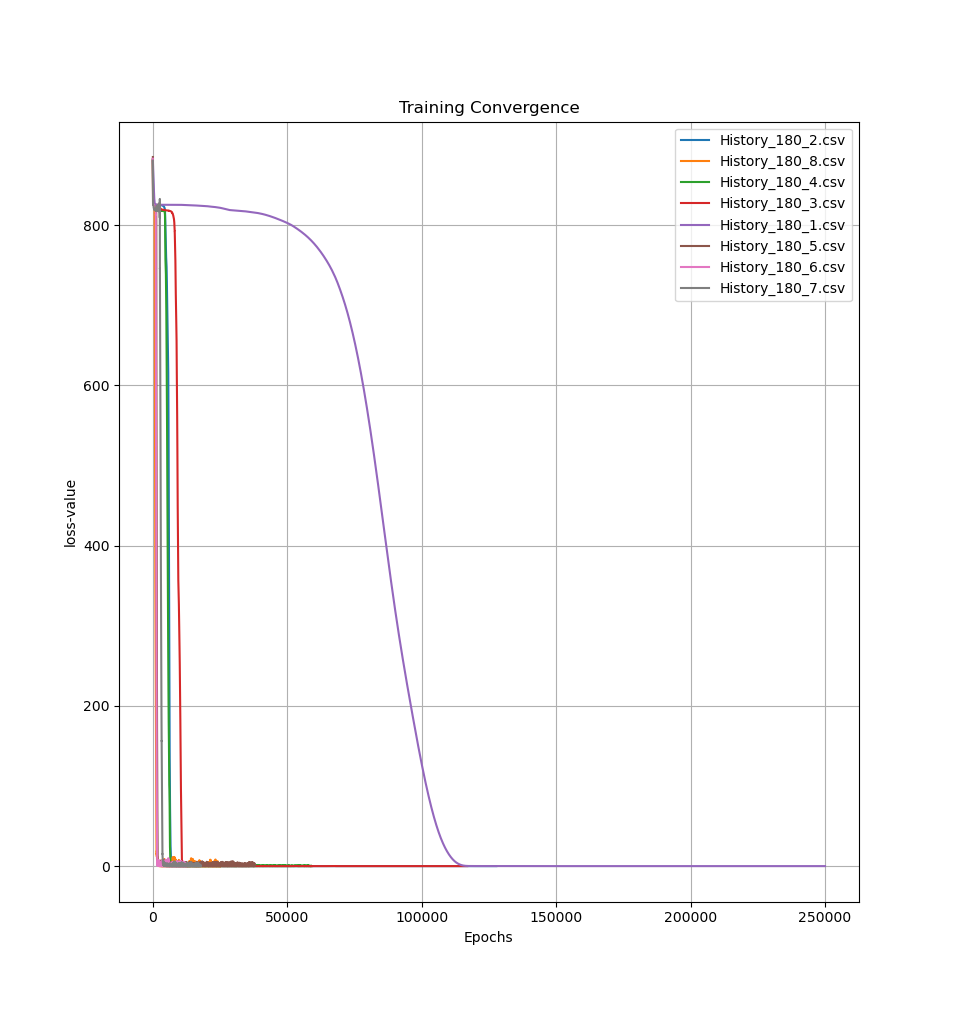
\includegraphics[scale=\size]{Width_180_Overview.png}
\newpage
At the beginning of the training iterations,
\\~\\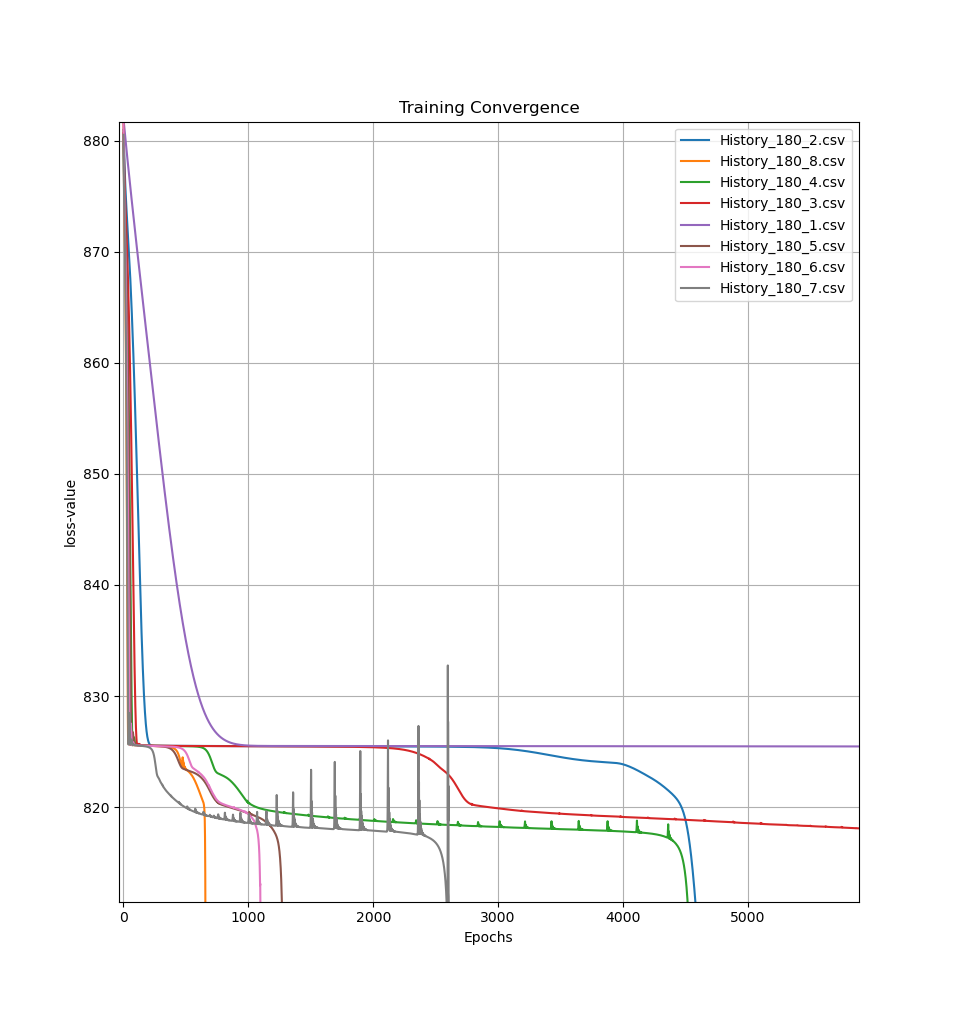
\includegraphics[scale=\size]{Width_180_Beginning.png}
\newpage
For the regions where many of the cases have converged,
\\~\\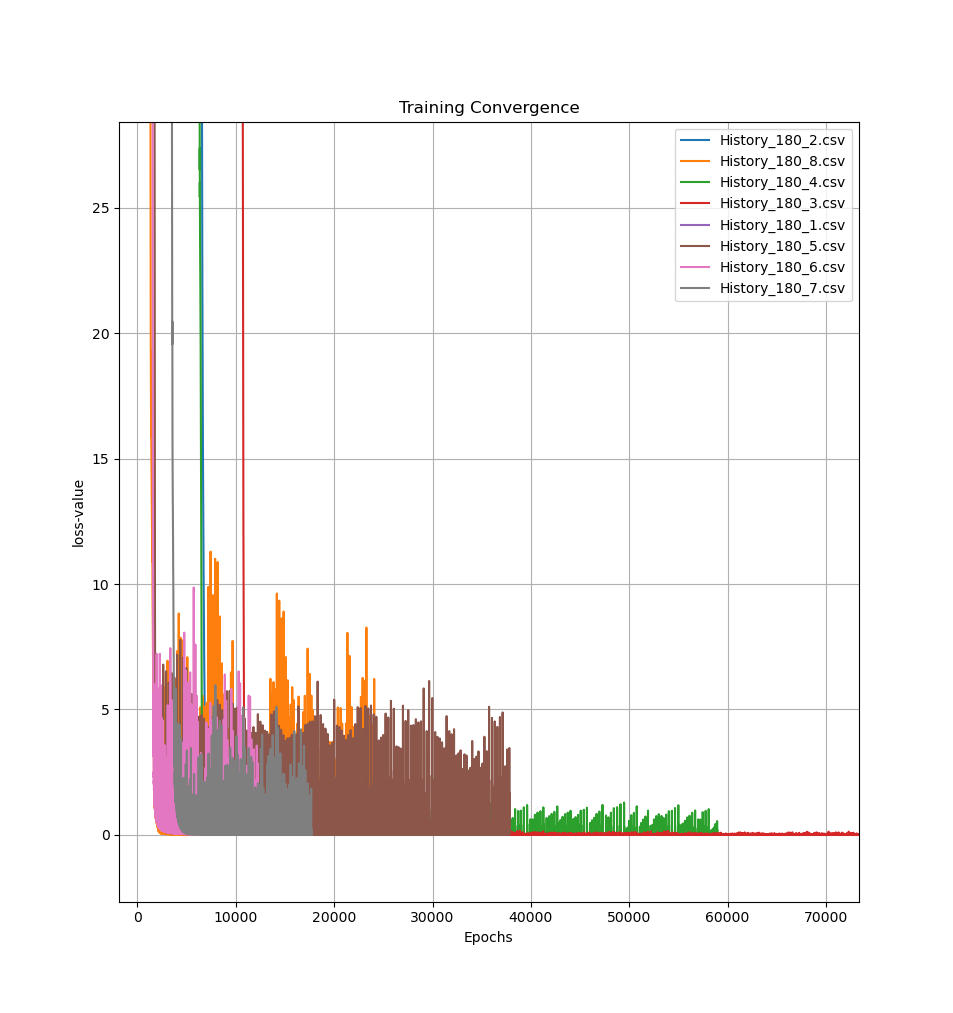
\includegraphics[scale=\size]{Width_180_Down.png}
%Seperator
%Seperator
\newpage
\subsection{Plots Across Constant Depth}
%Seperator
\subsubsection{2 Hidden Layers}
When there are $2$ hidden layers, an overview of the training curve,
\\~\\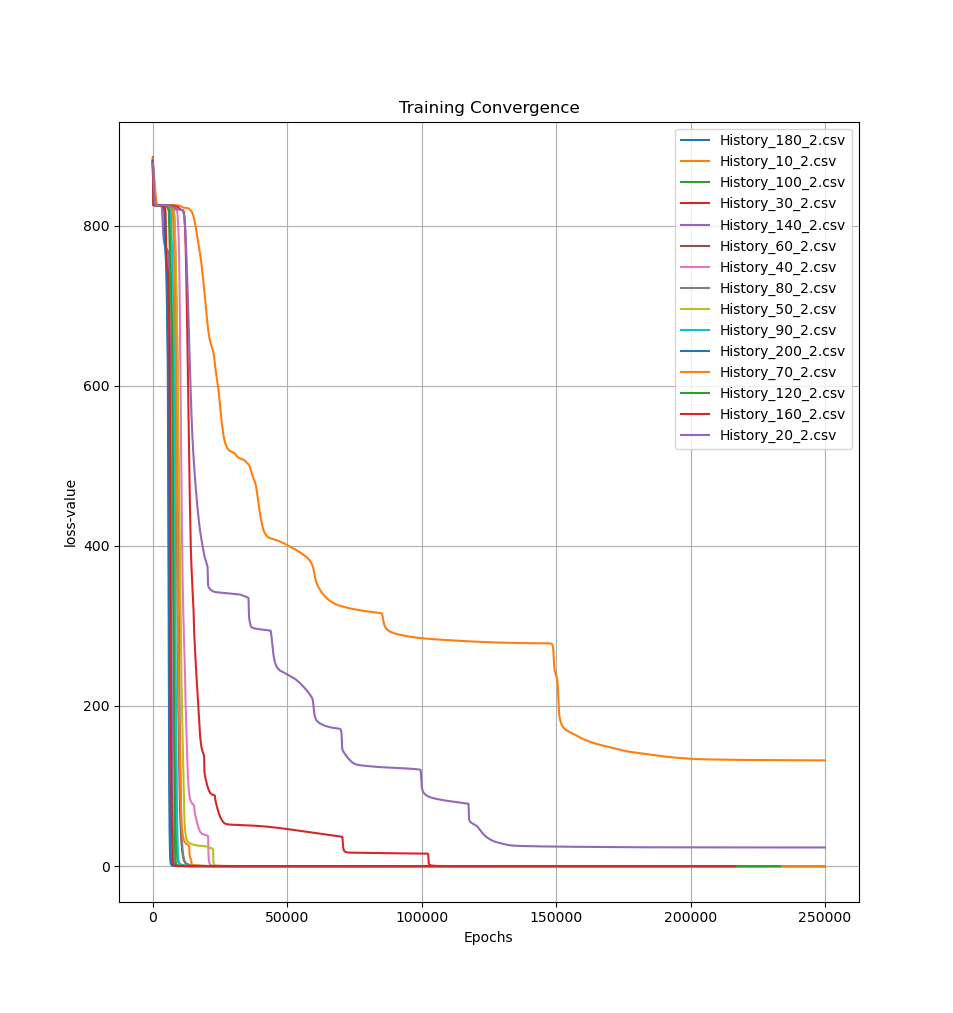
\includegraphics[scale=\size]{Depth_2_Overview.png}
\newpage
At the beginning of the training iterations,
\\~\\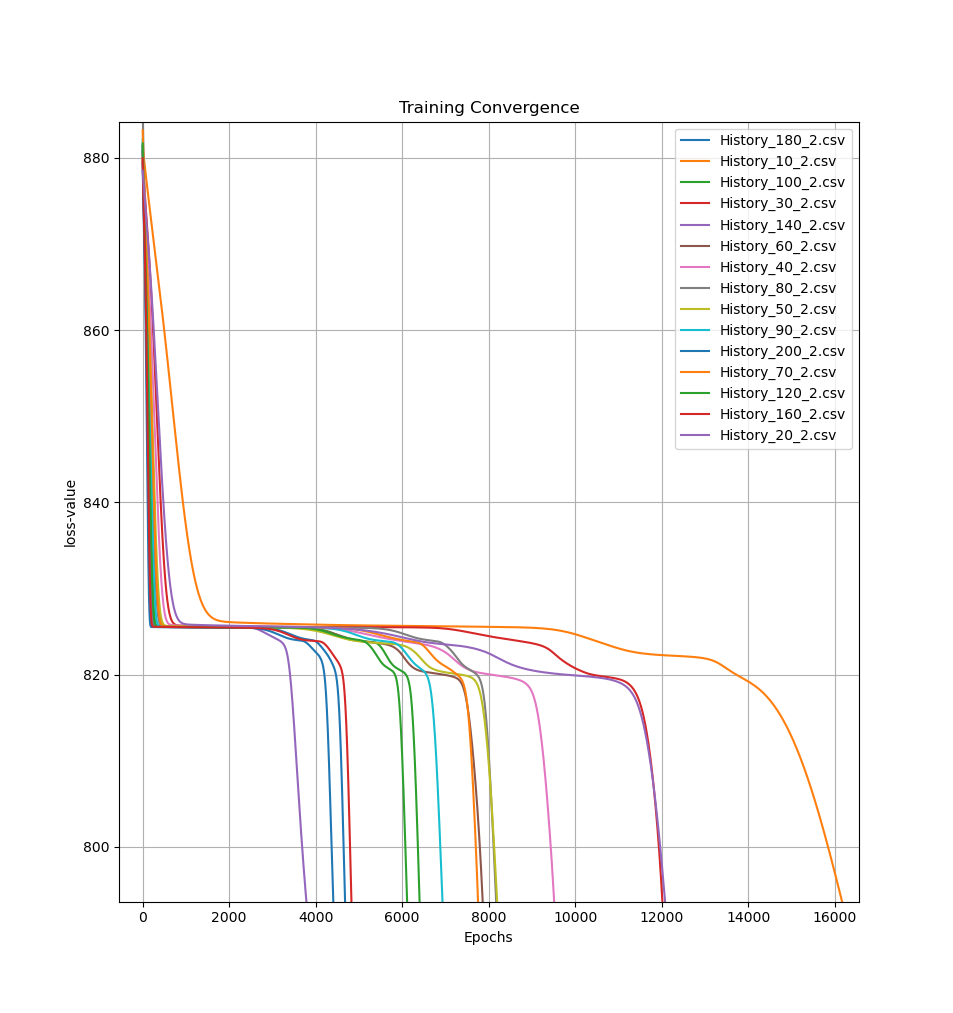
\includegraphics[scale=\size]{Depth_2_Beginning.png}
\newpage
For the regions where many of the cases have converged,
\\~\\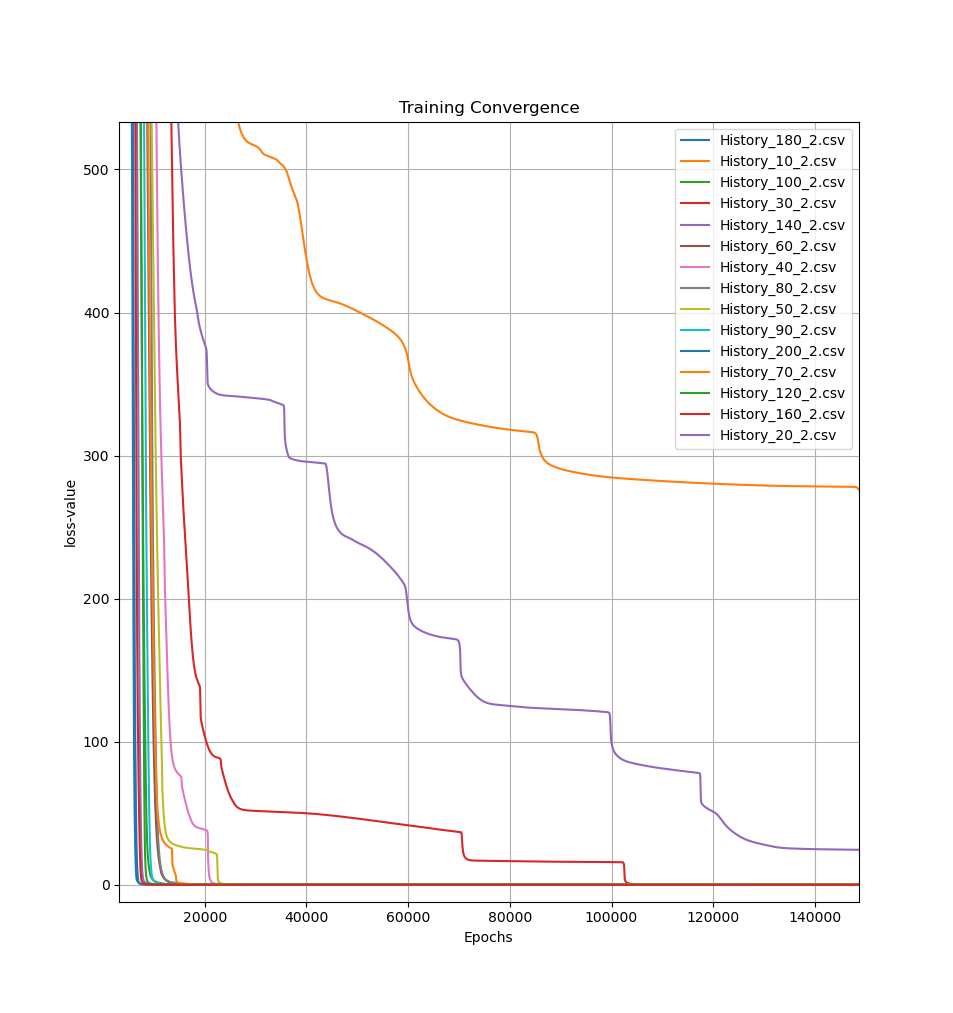
\includegraphics[scale=\size]{Depth_2_Down.png}
%Seperator
\newpage
\subsubsection{5 Hidden Layers}
When there are $5$ hidden layers, an overview of the training curve,
\\~\\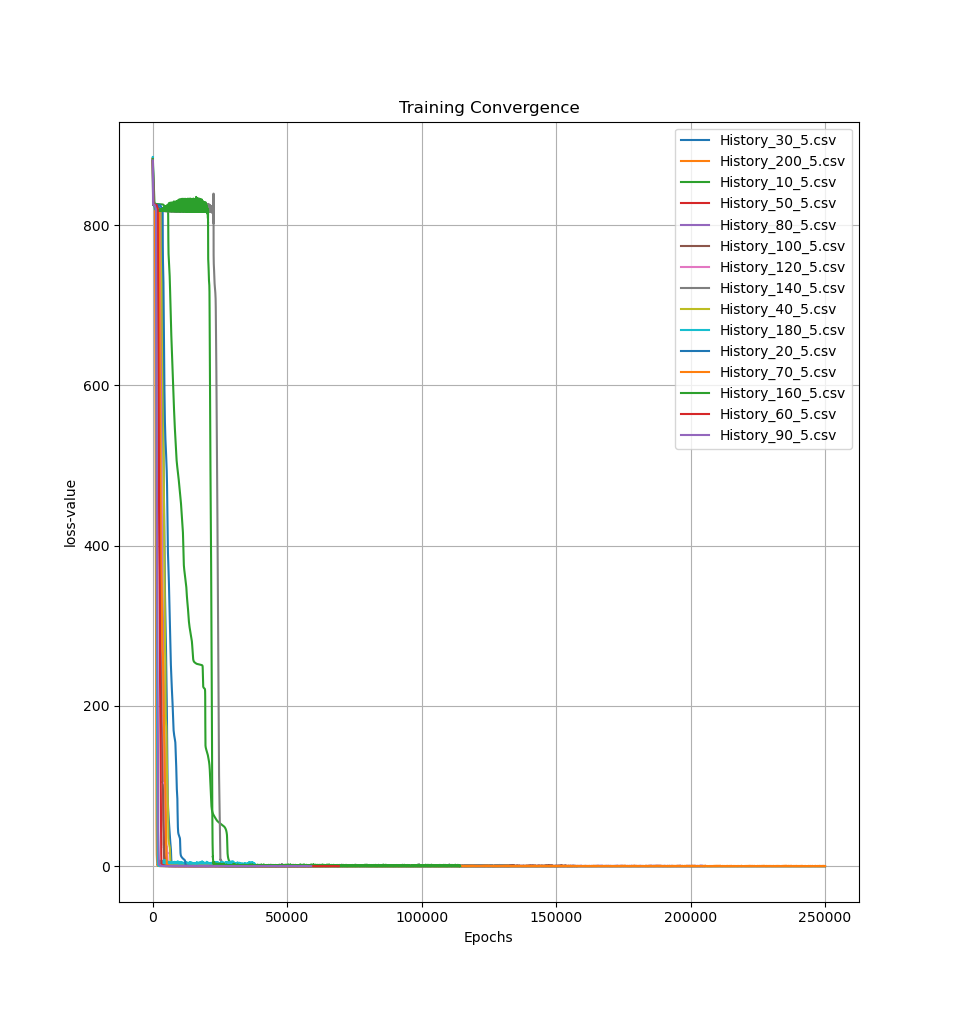
\includegraphics[scale=\size]{Depth_5_Overview.png}
\newpage
At the beginning of the training iterations,
\\~\\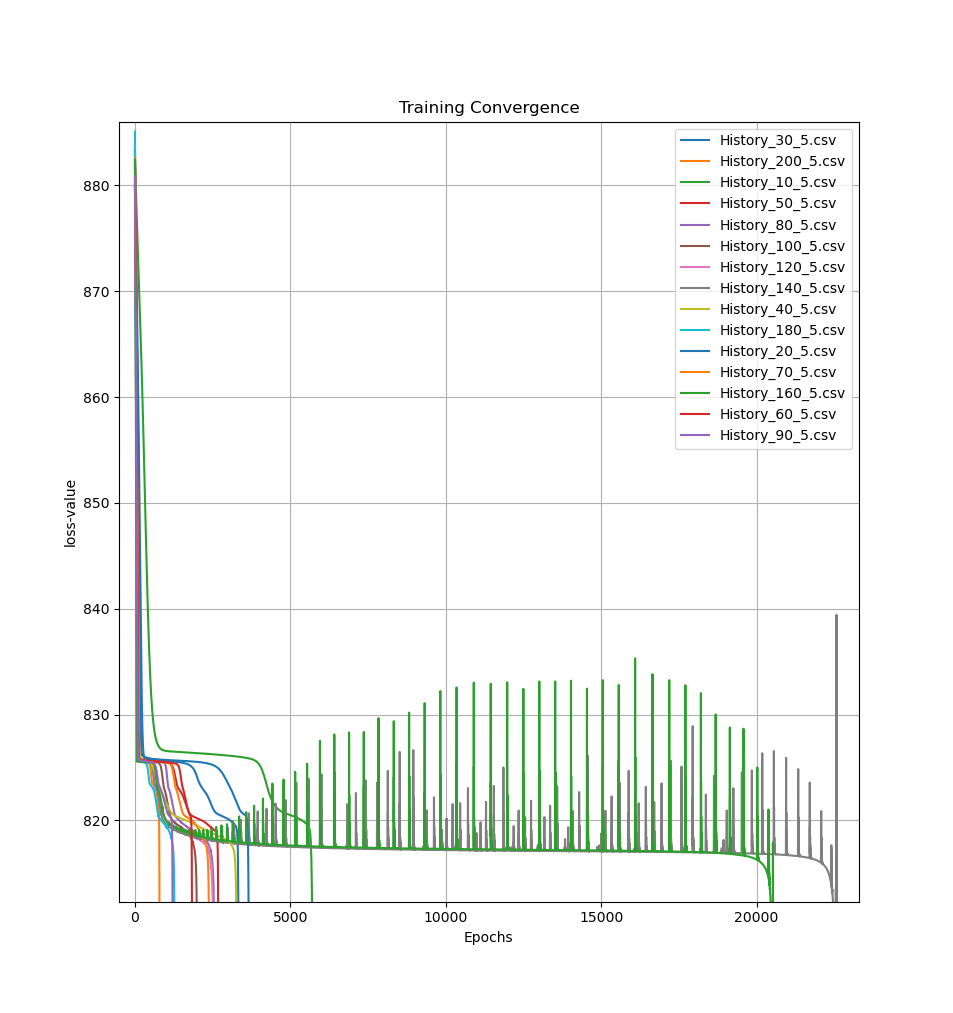
\includegraphics[scale=\size]{Depth_5_Beginning.png}
\newpage
For the regions where many of the cases have converged,
\\~\\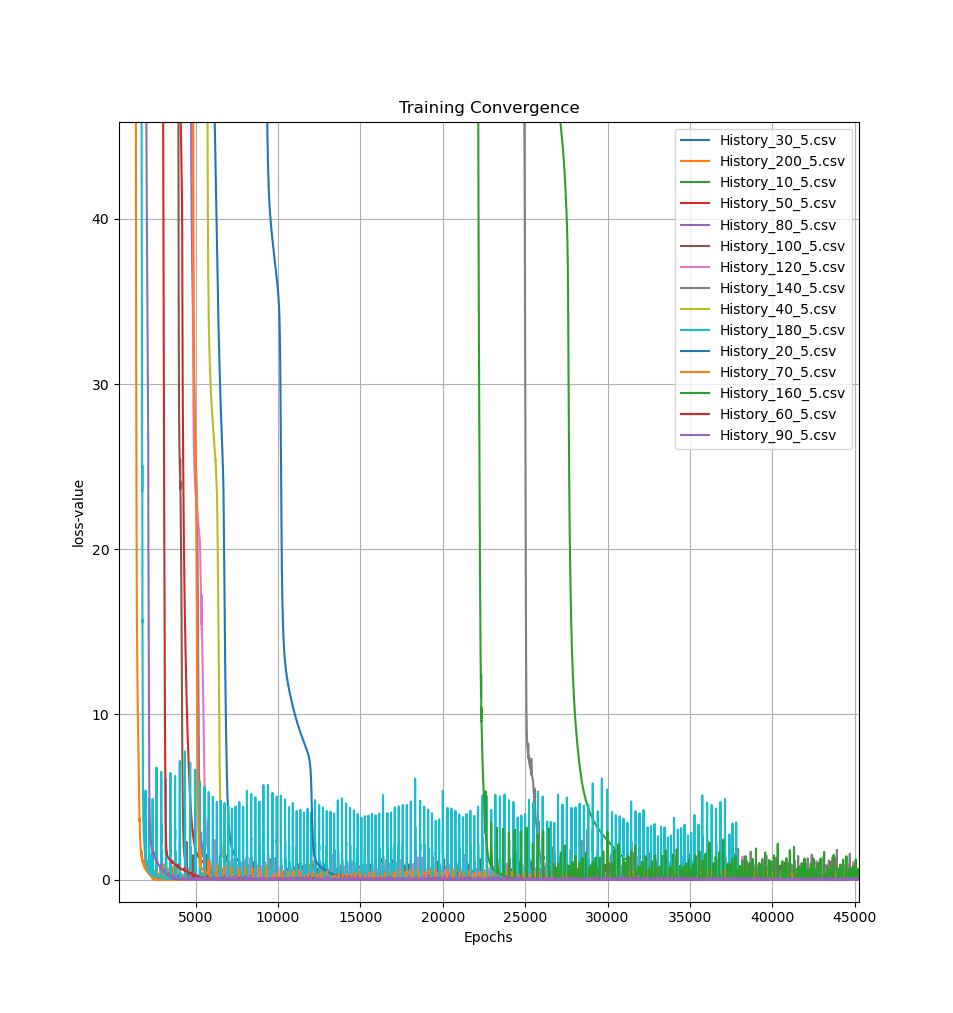
\includegraphics[scale=\size]{Depth_5_Down.png}
%Seperator
\newpage
\subsubsection{8 Hidden Layers}
When there are $8$ hidden layers, an overview of the training curve,
\\~\\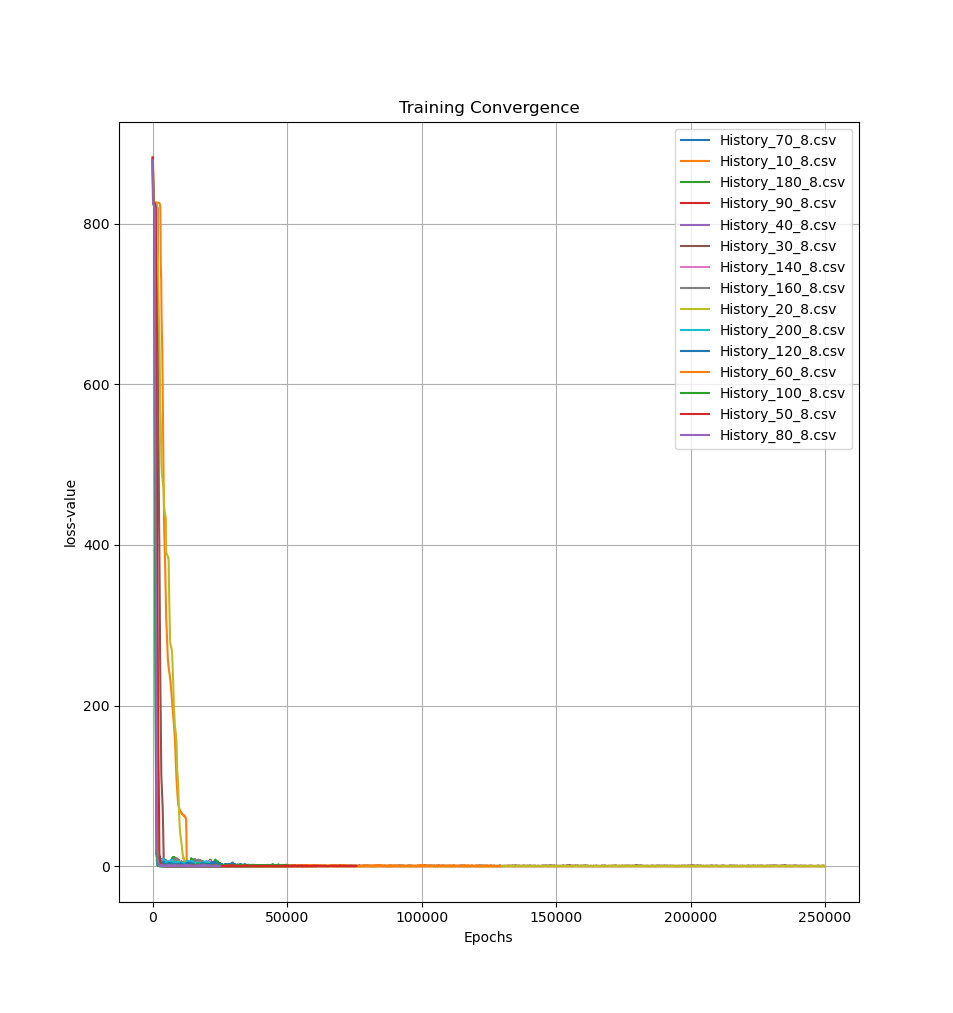
\includegraphics[scale=\size]{Depth_8_Overview.png}
\newpage
At the beginning of the training iterations,
\\~\\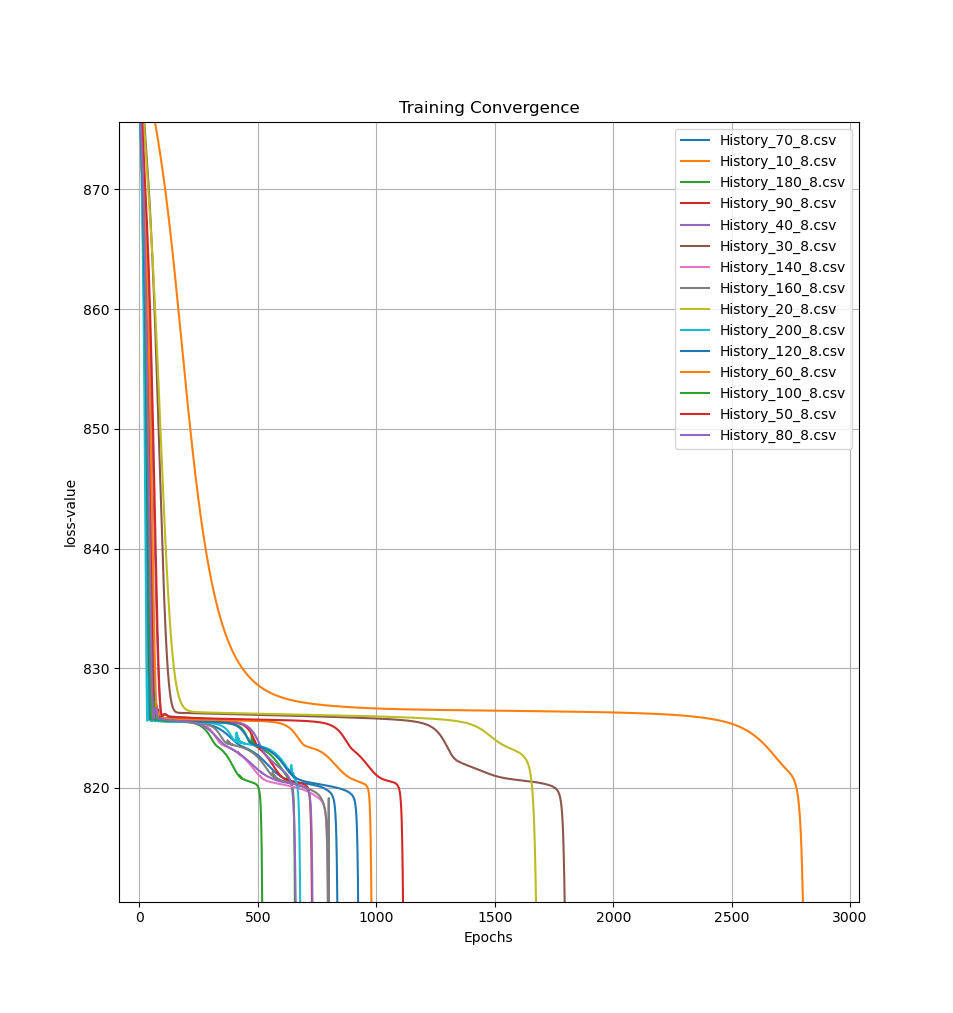
\includegraphics[scale=\size]{Depth_8_Beginning.png}
\newpage
For the regions where many of the cases have converged,
\\~\\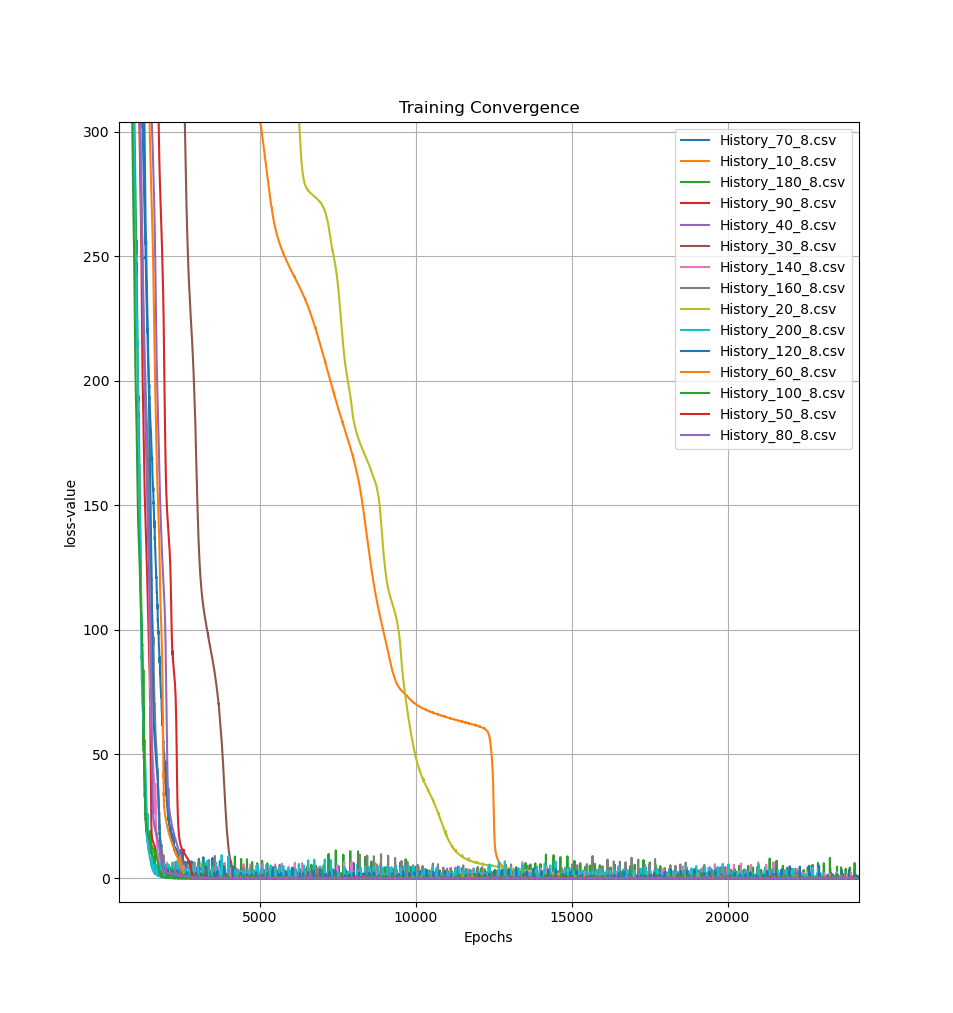
\includegraphics[scale=\size]{Depth_8_Down.png}
%Seperator
%Seperator
%Seperator
\section{Analysis}
\begin{comment}
\end{comment}
From the plots in the previous section it could be seen that for a fixed number of nodes per hidden layer, a neural network with more hidden layers would generally converge faster than a neural network with less hidden layers. However, more hidden layers could affect the training stability of the neural network. More hidden layers in the case of around $9$ hidden layers for the $100$ nodes per layer neural network exhibits oscillations in its training curve.
\\~\\For a given number of hidden layers, the training process seems to converge faster for a larger number of nodes per hidden layer. However, just like before, as the number of hidden layers increase, the training process tends to become unstable. Together with the previous paragraph, the results here show that "larger" neural networks with more nodes per hidden layer and more hidden layers tend to converge faster for across its training iterations but tend to become less stable.
\\~\\Note that the results here are somewhat non-unique. The neural network given a different set of initial conditions can converge to a different local minima in its loss-function. However, the chances of this is quite small when considering the overall training curve. There are many instances for different cases where the training curve "levels"  for a while before dropping again. Given that for a large number of training iterations $\approx 50000$ the loss-function for many of the cases have not changed substantially, it seems that the results presented here are truly the converged results of the training process.

%Seperator
%Seperator
%Seperator
\section{Further Development}
\begin{comment}
\end{comment}
More computational rescources are necessary. A total computational of $\approx31$ hours was needed to solve all the cases. It would be useful if the testing was faster than this.
%Seperator
%Seperator
%Seperator
\section{Appendix}
\begin{comment}
\end{comment}
%Seperator
%Seperator
\subsection{Tabulated Error}
The Error of the Neural Network over its domain is tabulated below, wherein * represents convergence of the training process,
\\~\\\begin{longtable}{|m{\stabsize}|m{\stabsize}|m{\tabsize}|m{\tabsize}|m{\tabsize}|m{\mtabsize}|}
\hline
Width & Depth & Average Error & Maximum Error & $L^2$ & * \\ \hline
10 & 1 & 0.8152537558846409 & 2.13137414800375 & 1.0034338898759056 & False \\ \hline  
10 & 2 & 0.46732206884968724 & 2.40067252361467 & 0.7380401189755383 & True \\ \hline  
10 & 3 & 0.1908407953661618 & 1.79960121859884 & 0.36064996852242626 & True \\ \hline  
10 & 4 & 0.0007692687434791289 & 0.00436928167125616 & 0.0010455071432206753 & True \\ \hline  
10 & 5 & 0.0002401672311574387 & 0.00115183883141579 & 0.0003748023397015376 & True \\ \hline  
10 & 6 & 2.8481704620314817e-05 & 0.000121004314855622 & 3.7546732266198486e-05 & True \\ \hline  
10 & 7 & 0.00012114683556951888 & 0.000606668008475975 & 0.0001636466360419277 & True \\ \hline  
10 & 8 & 0.004751530923135064 & 0.0347233932361046 & 0.008223305330606301 & True \\ \hline  
10 & 9 & 4.3796649752435814e-05 & 0.000166833495129026 & 5.5473501786697096e-05 & True \\ \hline  
10 & 10 & 2.4289808396457617e-05 & 8.1708302459127e-05 & 2.8736991204903868e-05 & True \\ \hline  
20 & 1 & 0.32242124590497295 & 1.02086845093231 & 0.42859588899977225 & False \\ \hline  
20 & 2 & 0.3878135835798753 & 1.27676254944598 & 0.5782444960649846 & True \\ \hline  
20 & 3 & 2.5138566545164934e-05 & 0.000108523864033927 & 3.3172330549571025e-05 & True \\ \hline  
20 & 4 & 0.00019004256796588772 & 0.000526535191835986 & 0.00023274026358821416 & True \\ \hline  
20 & 5 & 5.310000280304146e-05 & 0.0003987310791147 & 7.953698347814135e-05 & True \\ \hline  
20 & 6 & 2.7220652182886987e-05 & 0.000119747225982625 & 3.5168735203081404e-05 & True \\ \hline  
20 & 7 & 1.3864120812793946e-05 & 0.000106377862135965 & 2.365001146182627e-05 & True \\ \hline  
20 & 8 & 0.0023277539468917986 & 0.0083324400143332 & 0.0034166511233091057 & True \\ \hline  
20 & 9 & 2.535800652900547e-05 & 0.000200564657272917 & 4.4162404129861535e-05 & True \\ \hline  
20 & 10 & 4.166559992762906e-05 & 0.00015655973172457 & 5.202201112274727e-05 & True \\ \hline  
30 & 1 & 0.08821478107184245 & 0.262819302470788 & 0.11763965612789706 & False \\ \hline  
30 & 2 & 4.5382843076693046e-05 & 0.00023867519389853 & 6.739174931354081e-05 & True \\ \hline  
30 & 3 & 1.9323084349015702e-05 & 0.000260291613589203 & 4.2238169493443414e-05 & True \\ \hline  
30 & 4 & 0.0005234944022202108 & 0.00163663980997919 & 0.0006487117098273719 & True \\ \hline  
30 & 5 & 0.00034940708548401785 & 0.00104466209940046 & 0.00043900385259274167 & True \\ \hline  
30 & 6 & 0.00040632762512430887 & 0.00104900293841381 & 0.0004924704106217703 & True \\ \hline  
30 & 7 & 3.182961629471591e-05 & 7.60618729374052e-05 & 3.8236836931527965e-05 & True \\ \hline  
30 & 8 & 1.3436066208815143e-05 & 7.50077791666914e-05 & 1.93118169737034e-05 & True \\ \hline  
30 & 9 & 0.007732589958861411 & 0.0157313161279959 & 0.009094780772373866 & True \\ \hline  
30 & 10 & 2.9671977381217244e-05 & 0.000390352128168736 & 6.50758973695071e-05 & True \\ \hline  
40 & 1 & 0.023601359110570746 & 0.0790253899636069 & 0.031144814664306516 & False \\ \hline  
40 & 2 & 1.670831044352382e-05 & 6.61644300485875e-05 & 2.3852497763432287e-05 & True \\ \hline  
40 & 3 & 2.563275390853715e-06 & 1.2265365766595e-05 & 3.3260589342779997e-06 & True \\ \hline  
40 & 4 & 5.395511892754644e-06 & 2.62375536943527e-05 & 7.509388913093967e-06 & True \\ \hline  
40 & 5 & 3.7335745189558596e-06 & 2.34757088715121e-05 & 5.639711550778892e-06 & True \\ \hline  
40 & 6 & 2.3553560890932315e-05 & 0.000153416907444193 & 3.743339603956416e-05 & True \\ \hline  
40 & 7 & 1.2484831166395327e-05 & 4.12049509912471e-05 & 1.5179744468017645e-05 & True \\ \hline  
40 & 8 & 0.0003565596214747697 & 0.00130394517346932 & 0.0004544238499963453 & True \\ \hline  
40 & 9 & 1.4487596416754016e-05 & 0.000110641219748686 & 2.219760645737201e-05 & True \\ \hline  
40 & 10 & 1.8031848781365333e-05 & 0.00021184046500089 & 3.5092860611831794e-05 & True \\ \hline  
50 & 1 & 7.802233067599419e-05 & 0.0002548264446669 & 9.757448625430322e-05 & False \\ \hline  
50 & 2 & 5.6696374476304174e-05 & 0.000172970853218324 & 6.834275225742559e-05 & True \\ \hline  
50 & 3 & 1.3854532882666202e-05 & 5.06181256518801e-05 & 1.7310265272697606e-05 & True \\ \hline  
50 & 4 & 0.0015926833535170881 & 0.00337603055432245 & 0.0017894306020543968 & True \\ \hline  
50 & 5 & 0.000163949126243482 & 0.000384973199108352 & 0.00019227573359408763 & True \\ \hline  
50 & 6 & 1.4722075285195223e-05 & 5.8422605995645e-05 & 1.9138752096402113e-05 & True \\ \hline  
50 & 7 & 6.955410704667722e-06 & 7.81186943465961e-05 & 1.2915889047961956e-05 & True \\ \hline  
50 & 8 & 0.00012774796674291884 & 0.000297708435831101 & 0.00014773214951676456 & True \\ \hline  
50 & 9 & 0.00025650212380270195 & 0.000885952459482642 & 0.0003158987592732621 & True \\ \hline  
50 & 10 & 0.00018260458059517936 & 0.000642163200071932 & 0.00022673939821963928 & True \\ \hline  
60 & 1 & 7.089185334679635e-05 & 0.000222744651184437 & 8.920998022017012e-05 & False \\ \hline  
60 & 2 & 1.0978396641199308e-05 & 5.30430557472705e-05 & 1.4789103517519177e-05 & True \\ \hline  
60 & 3 & 1.90767905026459e-05 & 0.000237284461531484 & 4.121316511821175e-05 & True \\ \hline  
60 & 4 & 0.00030445853749446893 & 0.00101257530672827 & 0.0003861302072256795 & True \\ \hline  
60 & 5 & 8.299082112331985e-06 & 8.59035345328607e-05 & 1.3827340610975432e-05 & True \\ \hline  
60 & 6 & 0.0001301896026504204 & 0.000376302044680088 & 0.000155009530113849 & True \\ \hline  
60 & 7 & 7.422120684234973e-05 & 0.000199863190835092 & 8.724577991750605e-05 & True \\ \hline  
60 & 8 & 0.00010961302619233954 & 0.000223290901440798 & 0.0001263181200391331 & True \\ \hline  
60 & 9 & 3.3316150733287184e-05 & 0.00028094911481924 & 5.213827582744374e-05 & True \\ \hline  
60 & 10 & 7.466586387078734e-05 & 0.000693836279312521 & 0.00012132902821277287 & True \\ \hline  
70 & 1 & 0.000101331134187303 & 0.000320531719928629 & 0.00012336109189767025 & False \\ \hline  
70 & 2 & 7.370943779847706e-05 & 0.000203075480709636 & 8.861633038006931e-05 & True \\ \hline  
70 & 3 & 0.00029995898439541156 & 0.000892205360022658 & 0.00036738396915875416 & True \\ \hline  
70 & 4 & 3.7683642568509117e-06 & 1.48171638150174e-05 & 5.028296719698748e-06 & True \\ \hline  
70 & 5 & 0.0026722937768958502 & 0.00900330996626186 & 0.0031069114844717144 & True \\ \hline  
70 & 6 & 2.0771436493453898e-05 & 4.62638040008567e-05 & 2.404276595457956e-05 & True \\ \hline  
70 & 7 & 2.256959384298785e-05 & 0.000110585611538205 & 3.11421960528224e-05 & True \\ \hline  
70 & 8 & 0.0012510220465788429 & 0.00352620447842522 & 0.0015416825989355949 & True \\ \hline  
70 & 9 & 6.524843343291979e-05 & 0.000232849383486222 & 7.701250390056265e-05 & True \\ \hline  
70 & 10 & 0.0003532392526107973 & 0.001300506035534 & 0.00044973088184546695 & True \\ \hline  
80 & 1 & 0.00030808570452429826 & 0.00108478698864412 & 0.00041909224184128455 & True \\ \hline  
80 & 2 & 8.731362301823716e-06 & 5.72629691495408e-05 & 1.3788044607787769e-05 & True \\ \hline  
80 & 3 & 1.6023238323433585e-06 & 8.00568296499549e-06 & 2.139185127904659e-06 & True \\ \hline  
80 & 4 & 2.609421846478817e-06 & 1.3210295721322e-05 & 3.2850171963644037e-06 & True \\ \hline  
80 & 5 & 4.207377130469872e-06 & 2.59555384372057e-05 & 5.744228970434552e-06 & True \\ \hline  
80 & 6 & 0.0004412400796118111 & 0.0009436804229912 & 0.00051467100759637 & True \\ \hline  
80 & 7 & 0.000146481741136047 & 0.000406815943005068 & 0.00017349732664253978 & True \\ \hline  
80 & 8 & 0.00019979398131831193 & 0.000450301717203727 & 0.00022151523639277779 & True \\ \hline  
80 & 9 & 6.16641740467857e-05 & 0.000282448488100329 & 8.092466318053287e-05 & True \\ \hline  
80 & 10 & 0.00015606020463065722 & 0.000853096320268198 & 0.00021790347652608254 & True \\ \hline  
90 & 1 & 0.00022463606016048915 & 0.000695187516274398 & 0.00028838750822420765 & True \\ \hline  
90 & 2 & 2.1155681102938426e-05 & 7.59178611584588e-05 & 2.523857860771383e-05 & True \\ \hline  
90 & 3 & 2.2341899282132325e-06 & 2.18168550012443e-05 & 3.7637143686637415e-06 & True \\ \hline  
90 & 4 & 5.138697318102798e-05 & 0.000173899311146197 & 6.113837177561555e-05 & True \\ \hline  
90 & 5 & 5.4765732707173995e-05 & 0.000198799696649488 & 6.441231994196011e-05 & True \\ \hline  
90 & 6 & 2.3185399483918814e-05 & 0.000175801358075045 & 3.497501159847632e-05 & True \\ \hline  
90 & 7 & 0.0012367682207363698 & 0.00599191871324489 & 0.0017579914403204925 & True \\ \hline  
90 & 8 & 0.00014440833165011457 & 0.000325174248495763 & 0.0001682517453087211 & True \\ \hline  
90 & 9 & 5.6315448115962853e-05 & 0.000469485576283457 & 8.421072158418205e-05 & True \\ \hline  
90 & 10 & 0.0005438385986198327 & 0.00354651932264582 & 0.0007940492260901564 & True \\ \hline  
100 & 1 & 0.0002506940463304611 & 0.00224170670803936 & 0.0004448086241880708 & True \\ \hline  
100 & 2 & 5.209917021467555e-06 & 5.73529915715021e-05 & 1.008750996262275e-05 & True \\ \hline  
100 & 3 & 6.355312542911002e-05 & 0.000161550950225298 & 7.510527433452532e-05 & True \\ \hline  
100 & 4 & 3.1913179109987215e-06 & 1.61504172719873e-05 & 4.357377777460939e-06 & True \\ \hline  
100 & 5 & 1.1818416482806106e-05 & 4.78883052004164e-05 & 1.5846768432046913e-05 & True \\ \hline  
100 & 6 & 1.1808861924760127e-05 & 0.000127824277750044 & 2.106173184635491e-05 & True \\ \hline  
100 & 7 & 4.0109206907624956e-05 & 0.000348112789247512 & 6.713868053306532e-05 & True \\ \hline  
100 & 8 & 2.5091527878366393e-05 & 0.000254099344333181 & 4.174008071250583e-05 & True \\ \hline  
100 & 9 & 0.0031890839097906813 & 0.0143402811512079 & 0.003930690138999833 & True \\ \hline  
100 & 10 & 0.0001619284516581287 & 0.00154848021038889 & 0.0002933307432290376 & True \\ \hline  
100 & 1 & 0.0004296698164670647 & 0.000918595392271904 & 0.0004654266822302708 & True \\ \hline  
120 & 1 & 0.0001871438542712235 & 0.00183130161858536 & 0.0003212712548346149 & True \\ \hline  
120 & 2 & 3.3498903110835344e-06 & 2.11480538250264e-05 & 4.6280649836656564e-06 & True \\ \hline  
120 & 3 & 3.5633508675039556e-06 & 1.61195236101364e-05 & 4.584348674424251e-06 & True \\ \hline  
120 & 4 & 2.3917573413252254e-06 & 8.72469203461179e-06 & 2.9290514791735785e-06 & True \\ \hline  
120 & 5 & 5.225015550659752e-06 & 2.12691675778309e-05 & 6.5842510981679896e-06 & True \\ \hline  
120 & 6 & 3.0332396683439623e-05 & 0.00029689038013192 & 4.7507061114692996e-05 & True \\ \hline  
120 & 7 & 0.0018315614249662104 & 0.00796593133336687 & 0.002504535568170179 & True \\ \hline  
120 & 8 & 0.00012423512889700786 & 0.000494543663868363 & 0.00015385829764550838 & True \\ \hline  
140 & 1 & 0.00022918603376477815 & 0.00241370919211636 & 0.0003923932705395574 & True \\ \hline  
140 & 2 & 4.702862019374939e-06 & 4.55223263591265e-05 & 7.483099745370964e-06 & True \\ \hline  
140 & 3 & 1.3823951927667768e-05 & 4.07283464776143e-05 & 1.6350330383230615e-05 & True \\ \hline  
140 & 4 & 5.537473482925887e-06 & 5.70867712230694e-05 & 9.331684926461868e-06 & True \\ \hline  
140 & 5 & 7.291377772554732e-06 & 4.09256530771174e-05 & 9.838074059259181e-06 & True \\ \hline  
140 & 6 & 0.0009313928258801021 & 0.00429885205212011 & 0.0011714139039855143 & True \\ \hline  
140 & 7 & 0.00023915384527703617 & 0.000855739216087503 & 0.00028173530530391726 & True \\ \hline  
140 & 8 & 7.621240594467492e-05 & 0.000733783284823986 & 0.00014166358101879497 & True \\ \hline  
160 & 1 & 0.0006715736236207977 & 0.00103872142208417 & 0.0007372739694779137 & True \\ \hline  
160 & 2 & 1.0135981095218278e-05 & 5.92097182812168e-05 & 1.6832621664997018e-05 & True \\ \hline  
160 & 3 & 1.9386788461564104e-06 & 7.30807968030156e-06 & 2.511847662261138e-06 & True \\ \hline  
160 & 4 & 0.00019979555494656614 & 0.00100356834054915 & 0.00024755023204633546 & True \\ \hline  
160 & 5 & 2.1096622146623332e-05 & 0.000187791305037432 & 3.9547881065026715e-05 & True \\ \hline  
160 & 6 & 0.00011040155964962406 & 0.000974616815307972 & 0.0002101582287929308 & True \\ \hline  
160 & 7 & 8.877681077445051e-05 & 0.00118044227625891 & 0.0002011155906734561 & True \\ \hline  
160 & 8 & 0.000358343598941495 & 0.00404490285880321 & 0.0006858981721830683 & True \\ \hline  
180 & 1 & 0.000187405099336724 & 0.000729388484860483 & 0.00023309415985446532 & True \\ \hline  
180 & 2 & 8.496386556834278e-06 & 3.08327872018399e-05 & 1.0729839800211035e-05 & True \\ \hline  
180 & 3 & 0.00020416008471271172 & 0.000374009306611356 & 0.00023096358326257375 & True \\ \hline  
180 & 4 & 4.4287682381592465e-06 & 2.72614439769114e-05 & 6.234111240716437e-06 & True \\ \hline  
180 & 5 & 5.827597308709861e-05 & 0.00030255514923816 & 7.913024540380631e-05 & True \\ \hline  
180 & 6 & 0.0006561078429090557 & 0.00190377815051113 & 0.00080359775947715 & True \\ \hline  
180 & 7 & 0.000133736706835136 & 0.00129274827204773 & 0.00023958926020161358 & True \\ \hline  
180 & 8 & 0.00012576088584998458 & 0.00122354413787784 & 0.0002369410739528437 & True \\ \hline  
200 & 1 & 0.002073784070681088 & 0.00522902386972479 & 0.0025722808108057287 & True \\ \hline  
200 & 2 & 1.7065095809288207e-05 & 0.000121949170984958 & 2.940195766394337e-05 & True \\ \hline  
200 & 3 & 1.3144118357333672e-05 & 4.18022434156562e-05 & 1.739923165538816e-05 & True \\ \hline  
200 & 4 & 4.115715028307488e-05 & 0.000246057083590934 & 5.3755061131253186e-05 & True \\ \hline  
200 & 5 & 1.0528866435052094e-05 & 0.000104043922716901 & 1.8009789214151682e-05 & True \\ \hline  
200 & 6 & 0.0004889039753029384 & 0.00183038005933334 & 0.0006179715818090077 & True \\ \hline  
200 & 7 & 0.00013040624127057853 & 0.000486730237933664 & 0.00015745285441057832 & True \\ \hline  
200 & 8 & 0.00021859978863896366 & 0.00202711053996119 & 0.00036371557013522486 & True \\ \hline



\end{longtable}
%Seperator
%Seperator
%Seperator
\end{center}

\end{document}
